\documentclass{article}

\usepackage{fancyhdr}
\usepackage{extramarks}
\usepackage{amsmath}
\usepackage{amsthm}
\usepackage{amsfonts}
\usepackage{tikz}
\usepackage[plain]{algorithm}
\usepackage{algpseudocode}
\usepackage{chngcntr}
\usepackage{mathtools}
\usepackage[utf8]{inputenc}
\usepackage[english]{babel}
\usepackage{thmtools}
\usepackage{mathrsfs}
\usepackage{enumitem}

\declaretheoremstyle[headfont=\scshape,postheadspace=\newline]{mystyle}
\declaretheorem[style=mystyle]{theorem}

\usetikzlibrary{automata,positioning}

%
% Basic Document Settings
%

\topmargin=-0.45in
\evensidemargin=0in
\oddsidemargin=0in
\textwidth=6.5in
\textheight=9.0in
\headsep=0.25in

\linespread{1.1}

\pagestyle{fancy}
\lhead{\hmwkAuthorName}
\chead{\hmwkTitle}
\rhead{\firstxmark}
\lfoot{\lastxmark}
\cfoot{\thepage}

\renewcommand\headrulewidth{0.4pt}
\renewcommand\footrulewidth{0.4pt}

\setlength\parindent{0pt}

%\newtheorem{theorem}{Theorem}[section]
\newtheorem{corollary}{Corollary}[theorem]
\newtheorem{lemma}[theorem]{Lemma}
\theoremstyle{definition}
\newtheorem{definition}{Definition}[section]


%
% Create Problem Sections
%

\newcommand{\enterProblemHeader}[1]{
}

\newcommand{\exitProblemHeader}[1]{
    \nobreak\extramarks{#1 (continued)}{#1 continued on next page\ldots}\nobreak{}
    \stepcounter{#1}
    \nobreak\extramarks{#1}{}\nobreak{}
}

\setcounter{secnumdepth}{0}
\newcounter{partCounter}
\newcounter{homeworkProblemCounter}
\setcounter{homeworkProblemCounter}{1}

%
% Homework Problem Environment
%
% This environment takes an optional argument. When given, it will adjust the
% problem counter. This is useful for when the problems given for your
% assignment aren't sequential. See the last 3 problems of this template for an
% example.
%
\newenvironment{homeworkProblem}[1]{
    \section{#1}
    \setcounter{partCounter}{1}
    \setcounter{equation}{0}
    \setcounter{theorem}{0}
}

%
% Homework Details
%   - Title
%   - Due date
%   - Class
%   - Section/Time
%   - Instructor
%   - Author
%

\newcommand{\hmwkTitle}{MATH 2A: Differential Equations}
\newcommand{\hmwkDueDate}{}
\newcommand{\hmwkClass}{Discrete Mathematics}
\newcommand{\hmwkClassTime}{}
\newcommand{\hmwkClassInstructor}{}
\newcommand{\hmwkAuthorName}{\textbf{Edwin Njinimbam}}

%
% Title Page
%

\title{
    \vspace{2in}
    \textmd{\textbf{\hmwkClass\ \hmwkTitle}}\\
    \vspace{0.1in}\large{\textit{\hmwkClassInstructor\ \hmwkClassTime}}
    \vspace{3in}
}

\author{\hmwkAuthorName}
\date{}

\renewcommand{\part}[1]{\textbf{\large Part \Alph{partCounter}}\stepcounter{partCounter}\\}

%
% Various Helper Commands
%

% Useful for algorithms
\newcommand{\alg}[1]{\textsc{\bfseries \footnotesize #1}}

% For derivatives
\newcommand{\deriv}[2]{\frac{\mathrm{d}{#1}}{\mathrm{d}{#2}}}
\newcommand{\derivs}[2]{\frac{\mathrm{d}^2 {#1}}{\mathrm{d}{#2}^2}}

% For partial derivatives
\newcommand{\pderiv}[2]{\frac{\partial #1}{\partial #2}}
\newcommand{\pderivs}[2]{\frac{\partial^2 #1}{\partial #2^2}}

% Integral dx
\newcommand{\dx}{\mathrm{d}x}

% Alias for the Solution section header
\newcommand{\solution}{\textbf{\large Solution}}

% Probability commands: Expectation, Variance, Covariance, Bias
\newcommand{\E}{\mathrm{E}}
\newcommand{\Var}{\mathrm{Var}}
\newcommand{\Cov}{\mathrm{Cov}}
\newcommand{\Bias}{\mathrm{Bias}}

\newcommand{\ls} {\(\mathcal{LS}(A,\textbf{0})\)}
\newcommand{\nullspace}[1]{\mathcal{N}(#1)}
\newcommand{\p} {$\boxed{1}$~}
\newcommand*\Domain[1]{\in\mathbb{C}^{#1}}
\newcommand{\iu}{{i\mkern1mu}}

\counterwithin*{equation}{section}
\counterwithin*{equation}{subsection}

\newcommand{\matxx}[2] {
\begin{bmatrix}
  #1 \\
  #2 \\
\end{bmatrix}
}

\newcommand{\matxxx}[3] {
\begin{bmatrix}
  #1 \\
  #2 \\
  #3 \\
\end{bmatrix}
}

\newcommand{\matxxxx}[4] {
\begin{bmatrix}
  #1 \\
  #2 \\
  #3 \\
  #4 \\
\end{bmatrix}
}
\newcommand{\matxxxxx}[5] {
\begin{bmatrix}
  #1 \\
  #2 \\
  #3 \\
  #4 \\
  #5 \\
\end{bmatrix}
}

\newcommand{\matxxxxxx}[6] {
\begin{bmatrix}
  #1 \\
  #2 \\
  #3 \\
  #4 \\
  #5 \\
  #6 \\
\end{bmatrix}
}

\newcommand{\arrow}[1] {\xrightarrow[]{\text{#1}}}

\newcommand{\specialcell}[2][c]{%
  \begin{tabular}[#1]{@{}c@{}}#2\end{tabular}}

\newenvironment{solutionToProblem} {

  \bigskip

  \textbf{Solution}
}

\begin{document}

\begin{homeworkProblem}{Chapter1.1 \#17 Drag Race}
  \begin{solutionToProblem}
    Let us consider Alice and Kevin begin from a standing start in the race and
    they move foward with a constant acceleration. Let us denote \(A\) for Alice
    and \(K\) for Kevin then we can say that
    \[
      a(t) = k, \mbox{ where } k \mbox{ is a constant.}
    \]

    Then the \textit{velocity} is
    \[
      \begin{split}
        v(t) & = \int{a(t)dt} + C \\
        & = \int{k dt} + C \\
        & = kt + C
      \end{split}
      \]

      The initial velocity is zero, Thus, we get
      \[
        \begin{split}
          v(0) & = 0 \\
          k(0) + C & = 0 \\
          C & = 0
        \end{split}
      \]

      Therefore the velocity is \[v(t) = kt\]

      \bigskip

      Let us denote that
      \[
        \begin{split}
          s(t) & = \int{v(t)dt} + C_1 \\
          & = \int{kt dt} + C_1 \\
          & = \frac{kt^2}{2} + C_1
        \end{split}
      \]
        The constant value will be zero since our standing point is at the
        beginning of the race. Therefore,
        \[
          s(t) = \frac{1}{2}kt^2
        \]

        Now, the acceleration is the second derivative of the position function,
        or is the first derivative of the velocity function. Therefore,
        \[
          a = \deriv{v}{t} = k
        \]

        Let \(D\) represent the total distance of the racec and \(T\) be the
        time then we get
        \[
          D = s(t) = \frac{1}{2}aT^2
        \]

        Solving this equation for \(T\) to get
        \[
          T = \sqrt{\frac{2D}{a}}
        \]

        \bigskip

        For Kevin, when she has \(\frac{1}{4}\) left to go she has already
        traveled \(\frac{3}{4}\) of the entire distance \(D\), so we can express
        this as follows:
        \[
          \begin{split}
            t_{\frac{3}{4}} & = \sqrt{\frac{2\left( \frac{3}{4} \right)D}{a}} \\
            & = \sqrt{\frac{3}{4}}\sqrt{\frac{2D}{a}} \\
            & = \frac{\sqrt{3}}{2}T
          \end{split}
        \]

        Thus, the total time for Kevin to complete the race is,
        \[
          \begin{split}
            T & = t_{\frac{1}{4}} + t_{\frac{3}{4}} \\
            T & = 3 + \frac{\sqrt{3}}{2}T \\
            T\left( 1 - \frac{\sqrt{3}}{2} \right) & = 3 \\
            T \left( \frac{2 - \sqrt{3}}{2} \right) & = 3 \\
            T & = \frac{6}{2 - \sqrt{3}} \\
            T & = 6\left( 2 + \sqrt{3} \right)
          \end{split}
        \]

        Thus, \[T = 6\left( 2 + \sqrt{3} \right) \approx 22.3923 \mbox{ seconds for
            Kevin to finish the race.}\]

        Now, we need to find the time how long it takes for Alice to finish the
        race in a similar manner. When Alice has \(\frac{1}{3}\) to go her has
        already covered \(\frac{2}{3}\) of the total distance of the race.
        \[
          \begin{split}
            t_{\frac{2}{3}} & = \sqrt{\frac{2\left( \frac{2}{3} \right)D}{a}} \\
            & = \sqrt{\frac{2}{3}} \sqrt{\frac{2D}{a}} \\
            & = \sqrt{\frac{2}{3}}T
          \end{split}
        \]

        Therefore, the total time for Alice to complete the race is
        \[
          \begin{split}
            T & = t_{\frac{1}{3}} + t_{\frac{2}{3}} \\
            T & = 4 + \sqrt{\frac{2}{3}}T \\
            T \left( 1 - \sqrt{\frac{2}{3}} \right) & = 4 \\
            T\left( \frac{\sqrt{3} - \sqrt{2}}{\sqrt{3}} \right) & = 4 \\
            T & = \frac{4\sqrt{4}}{\sqrt{3} - \sqrt{2}} \\
            T & = 4\sqrt{3}\left( \sqrt{3} + \sqrt{2} \right) \\
            T & = 4\left( 3 + \sqrt{6} \right) \approx 21.798 \\
          \end{split}
        \]

        Thus, Alice wins by
        \[
          \begin{split}
            T & = 6\left( 2 + \sqrt{3} \right) - 4\left( 3 + \sqrt{6} \right)
            \\
            & = 6\sqrt{3} - 4\sqrt{6} \\
            \approx 0.594
          \end{split}
        \]

        Thus, Alice wins by \(\left( 6\sqrt{3} - 4\sqrt{6} \right)\) seconds.
  \end{solutionToProblem}
\end{homeworkProblem}

\pagebreak

\begin{homeworkProblem}{Chapter 1 B: Picard's Method}
  \begin{enumerate}[label=(\alph*)]
  \item  Use Picard's method with \(\psi_{0}(x) = 1\) to obtain the next four
    successive approximations of the solution to
    \[y^{\prime}(x) = y(x), \hspace{0.5cm} y(0) = 1\]
    Show that these approximations are just the partial sums of the Maclaurin
    series for the actual solution \(e^x\).

    \begin{solutionToProblem}
      Given that
      \begin{equation}
        y^{\prime}(x) = y(x), \hspace{0.5cm} y(0) = 1
      \end{equation}

      Also given that
      \begin{equation}
        f(x,y) = y(x)
      \end{equation}
      According to picards theorem, we have
      \begin{equation}
        \begin{split}
          \phi_{n+1}(x) & = y_0 + \int^{x}_{x_{0}}{f(t, \phi_{0}(t))}dt \\
          & = 1 + \int^{x}_{0}{1}dt \\
          & = 1 + x
        \end{split}
      \end{equation}

      \begin{equation}
        \begin{split}
          \phi_{2}(x) & = y_0 + \int^{x}_{0}f(t, \phi_1(t))dt \\
          & = 1 + \int^{x}_{0} f(t, \left( 1+t \right))dt \\
          & = 1 + x + \frac{x^2}{2}
        \end{split}
      \end{equation}

      \begin{equation}
        \begin{split}
          \phi_{3}(x) & = y_0 + \int^{x}_{0}f(t, \phi_2(t))dt \\
          & = 1 + \int^{x}_{0} f \left(t, \left( 1+t + \frac{t^2}{2} \right) \right)dt \\
          & = 1 + x + \frac{x^2}{2} + \frac{x^3}{6}
        \end{split}
      \end{equation}

      \begin{equation}
        \begin{split}
          \phi_{4}(x) & = y_0 + \int^{x}_{0}f(t, \phi_3(t))dt \\
          & = 1 + \int^{x}_{0}f \left( t, \left( 1 + t + \frac{t^2}{2} \right) \right)dt \\
          & = 1 + x + \frac{x^2}{2} + \frac{x^3}{6} + \frac{x^4}{24}
        \end{split}
      \end{equation}

      By observing the pattern as \(n\) goes, it is enough to say that
      \[
        \phi_{n}(x) = 1 + x + x^2 + \frac{x^2}{2} + \frac{x^3}{6} + \dots + \frac{x^n}{n!}
      \]

      This is the partial sum of the Maclaurian series of \(e^x\).
    \end{solutionToProblem}

  \item Use Picard's method with \(\psi+{0}(x) = 0\) to obtain the next
    three successive approximations of the solution to the nonlinear problem
    \[
      y^{\prime}(x) = 3x - \left[ y(x)^2 \right], \hspace{0.5cm} y(0) = 0
    \]
    Graph these approximations for \(0 \leq x \leq 1\).

    \begin{solutionToProblem}
      \setcounter{equation}{0}
      \begin{equation}
        \begin{split}
          y(x_1) & = y(x_0) + \int^{x}_{x_0}{f(x,y)dx} \\
          & = f(x,y) = 2x - y^2 \\
          y(0) & = 0
        \end{split}
      \end{equation}
      We assume that \(x_0 = 0, x_1 = 0.25\) then
      \begin{equation}
        \begin{split}
          \phi_1(x) & = y(0) + \int^{x}_{0}{\phi_0(x)dx} = 0 + \int^{x}_{0}{2x - 0}dx = x^2 \\
          \phi_2(x) & = y(0) + \int^{x}_{0}{\phi_1(x)dx} = 0 + \int^{x}_{0}{(2x - x^2)dx} = x^2 - =frac{x^3}{3} \\
          \phi_3(x) & = y(0) + \int^{x}_{0}{\phi_2(x)dx} = 0 + \int^{x}_{0}{(2x - x^2 + \frac{x^3}{3})dx} = x^2 - =frac{x^3}{3} + \frac{x^4}{12} \\
          \phi_4(x) & = y(0) + \int^{x}_{0}{\phi_3(x)dx} = 0 + \int^{x}_{0}{(2x - x^2 + \frac{x^3}{3} - \frac{x^4}{12})dx} = x^2 - =frac{x^3}{3} + \frac{x^4}{12} - \frac{x^5}{60} \\
        \end{split}
      \end{equation}
      If \(x = 0.25, \phi_1(x) = 0.0625, \phi_2(x) = 0.05729, \phi_3(x) =
      0.05761, \phi_4(x) = 0.0576009\).
      Thus, the better approximationn at \(x = 0.25\) is \(0.0576\).

      If \(x = 0.5, \phi_1(x) = 0.25, \phi_2(x) = 0.2083, \phi_3(x) =
      0.203125, \phi_4(x) = 0.21302\).

      If \(x = 0.75, \phi_1(x) = 0.5625, \phi_2(x) = 0.421875, \phi_3(x) =
      0.44824, \phi_4(x) = 0.605419\).

      \begin{center}
        \begin{figure}[h!]
          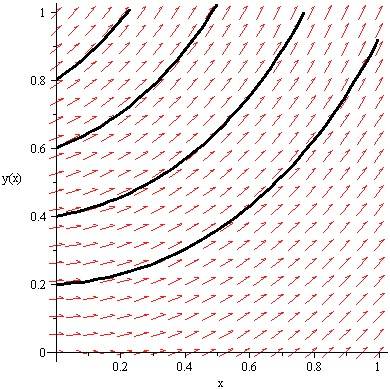
\includegraphics[width=7cm]{chap1b.jpg}
          \caption{}
          \label{fig:chap1b}
        \end{figure}
      \end{center}
    \end{solutionToProblem}

  \item In Problem 29 in Exercises 1.2, we showed that the initial value
    problem
    \[y^{\prime}(x) = 3\left[ y(x)\right]^{2/3}, y(2) = 0\]
    does not have a unique solution. Show that Picard's method beginning
    with \(\psi_{0}(x) = 0\) converges to the solution \(y(x) = 0\),
    whereas Picard's method beginning with \(\psi_{0}(x) = x - 2\)
    converges to the second solution \(y(x) = (x - 2)^{3}\).

    \begin{solutionToProblem}
      \setcounter{equation}{0}
      The given IVP can be written as
      \begin{equation}
        y^{\prime}(t) = f(x, y(x)) \mbox{ where } f(x,y(x)) = 3(y(x))^{2/3}
      \end{equation}

      The first iteration is given by

      \begin{equation}
        \begin{split}
          y_1(x) & = y(2) + \int^{x}_{2} f(u, y(2))du \\
          & = 0 + \int^{t}_{2} f(u, 0)du \\
          & = 0 + \int^{x}_{0} 0du = 0
        \end{split}
      \end{equation}
      If we repeat the procedure, then we get
      \begin{equation}
        y_2(x) = 0
      \end{equation}

      Thus, we get the trivial solution \(y(x) = 0\) for the IVP.

      \bigskip

      Suppose that
      \begin{equation}
        \phi_0(x) = x - 2
      \end{equation}

      Then the first iteration is given by
      \begin{equation}
        \begin{split}
          \phi_1(x) & = \phi_0(x) + \int^{x}_{2} f\left( u, \phi_0(x) \right)du \\
          & = x - 2 + \int^{x}_{2}f(u, x-2)du \\
          & = x - 2 + \int^{x}_{2}{3(x - 2)^{2/3}du} = x - 2 3 \frac{(x-2)^{5/3}}{5/3} \Bigm|_2^x \\
          & = x - 2 + \frac{9}{5}(x-2)^{5/3} = (x-2)\left( 1 + \frac{9}{5}(x-2)^{2/3} \right)
        \end{split}
      \end{equation}

      The second iteration is given by
      \begin{equation}
        \begin{split}
          \phi_2(x) & = \phi_0(x) + \int^{x}_{2}{\left( fu, \phi_1(x) \right)du} \\
          & = x - 2 + \int^{x}_{2}f\left( u, x-2 \right)du \\
          & = x - 2 + \int^{x}_{2}{x - 2 + \frac{9}{5}(x-2)^{5/3}du} = x - 2 + \left( \frac{(x-2)^2}{2} + \frac{9}{5}\frac{(x-2)^{8/3}}{8/3} \Bigm|^{x}_{2} \right) \\
          & = x - 2 =\frac{(x-2)^{2}}{2} + \frac{27}{40}(x-2)^{8/3}
        \end{split}
      \end{equation}
    \end{solutionToProblem}
  \end{enumerate}
\end{homeworkProblem}

\pagebreak

\begin{homeworkProblem}{The Phase Line}
  \begin{enumerate}[label=(\alph*)]
  \item The slopes in the direction field are all identical along horizontal
    lines.

    \begin{solutionToProblem}
    \end{solutionToProblem}
    
  \item New solutions can be generated from old ones by time shifting [i.e.,
    replacing \(y(t)\) with \(y(t-t_0)\).]

    \begin{solutionToProblem}
    \end{solutionToProblem}
        
  \item Sketch the phase line for \(y^{\prime} = (y - 1)(y - 2)(y - 3)\) and
    state the nature of its equilibria.

    \begin{solutionToProblem}
    \end{solutionToProblem}
    
  \item Use the phase line for \(y^{\prime} = -(y - 1)^{5/3}(y - 2)^2(y -
    3)\) to predict the asymtotic behavior as \(t \rightarrow \infty\) of the
    solution satisfying \(y(0) = 2.1\).
    \begin{solutionToProblem}
    \end{solutionToProblem}
    
  \item Sketch the phase line for \(y^{\prime} = y{\sin{y}}\) and state the
    nature of its equilibria.
    \begin{solutionToProblem}
    \end{solutionToProblem}
    
  \item Sketch the phase lines for \(y^{\prime} = y \sin{y} + 0.1\) and
    \(y^{\prime} = y\sin{y} - 0.1\). Discuss the effect of the small
    perturbation \(\pm 0.1\) on the equilibria.
    \begin{solutionToProblem}
    \end{solutionToProblem}
  \end{enumerate}
\end{homeworkProblem}

\pagebreak

\begin{homeworkProblem}{Chapter 4 A: Nonlinear Equations Solvable by First-Order Techniques}
  \begin{enumerate}[label=(\alph*)]
  \item
    \begin{solutionToProblem}
      
      The given equation can ben rewritten as
      
      \[
        \begin{split}
          2x\deriv{w}{x} - w + \frac{1}{w} & = 0 \\
          2x\deriv{w}{x} & = w - \frac{1}{w} \\
          \frac{1}{w - 1/w}dw & = \frac{1}{2x}dx
        \end{split}
      \]

      Therefore we get
      \[
        \frac{1}{2} \int{\left( \frac{1}{w^2 - 1}2w \right) dw} = \frac{1}{2} \int{\frac{1}b{2}dx}
      \]

      That is
      \[
        \begin{split}
          \ln{w^2 - 1} & = \ln{\left| x \right| + C} \\
          w^2 - 1 & = x + C \\
          w & = \deriv{y}{x} = \sqrt{x + 1}
        \end{split}
      \]

      Thus, we obtain

      \[
        y = \int{\left( x + 1 \right)^{\frac{1}{2}}}dx = \frac{1}{2\sqrt{x+1}} + C
      \]
    \end{solutionToProblem}
  \item
    
    \begin{solutionToProblem}
      \[
        \begin{split}
          (2y)(w)\deriv{w}{y} & = 1 + w^2 \\
          2y\deriv{w}{y} & = \frac{1}{w} + w = \frac{w^2 + 1}{w} \\
        \end{split}
      \]

      This becomes
      \[
        \frac{1}{2}\int{1}{\left( w^2 + 1 \right) (2w)dw} = \frac{1}{2} \int{\frac{1}{y}}dy
      \]

      Then we obtain
      \[
        \begin{split}
          w & = \sqrt{y - 1} + C
        \end{split}
      \]

      \[
        \begin{split}
          \int{\frac{1}{\sqrt{y - 1}}dy} = \int{dx}
          \sqrt{y - 1} & = 2x + C_1
        \end{split}
      \]

      Thus we obtain
      \[
        y_1 = 1 + 4x^2 + C
      \]

      Then we need to have another equation.
      \[
        2yw\deriv{w}{y} = -yw
        2\deriv{w}{y} = -\frac{yw}{yw} = -1
      \]

      \[
        \begin{split}
          \int{dw} & = -\frac{1}{2}\int{dy} \\
          -2 \int{\frac{1}{y}dy} & = \int{dx}
        \end{split}
      \]

      This becomes
      \[
        \begin{split}
          -2\ln{\left| y \right|} & = x + C \\
          \ln{\left| y \right|} & = -\frac{1}{2}x + C
        \end{split}
      \]

      Thus, we get
      \[
        y_2 = Ce^{-\frac{x}{2}}
      \]
    \end{solutionToProblem}

  \item \textbf{Suspended Cable.}
    \begin{solutionToProblem}
      \setcounter{equation}{0}
      The given differential equation is
      \begin{equation}
        y^{\prime\prime} = \frac{1}{a}\sqrt{1 + \left( \deriv{y}{x} \right)^2}; \hspace{0.5cm} y(0) = a, \hspace{0.5cm} y^{\prime}(0) = 0, \hspace{0.2cm} \mbox{ where } a (\neq 0) \mbox{ is a constant.}
      \end{equation}

      Let \(v = y^{\prime}\) then we can say that \(\deriv{v}{x} =
      y^{\prime\prime}\)
      
      Now, we solve
      \begin{equation}
        \begin{split}
          \deriv{v}{x} & = \frac{1}{a}\sqrt{1 + v^2} \\
          \int{\frac{dv}{\sqrt{1 + v^2}}} & = a\int{dx} \\
        \end{split}
      \end{equation}

      This becomes
      \begin{equation}
        \ln{\sqrt{1+v^2} + v} = ax
      \end{equation}

      Thus, this is enough reason to say that
      \[
        \begin{split}
          x^{\prime}(0) & = 0 \\
        \end{split}
      \]
      This means \(C = 0\).

      Therefore

      \begin{equation}
        \begin{split}
          \ln{\sqrt{1 + v^2} + v} & = ax \\
          \sqrt{1 + v^2} + v & = e^{ax} \\
          \left( -\sqrt{1 + v^2} \right) & = \left( v - e^{ax} \right)^2 \\
          v & = \frac{e^{2ax} - 1}{2e^{ax}} = \frac{1}{2}\left[ e^{ax} - e^{-ax}\right]
        \end{split}
      \end{equation}

      \begin{equation}
        \begin{split}
          \deriv{y}{x} & = \frac{1}{2}\left( e^{ax} - e^{-ax}\right) \\
          \int{dy} & = \frac{1}{2}\int{\left( e^{ax} - e^{-ax} \right)dx} \\
          y & = \frac{1}{2}\frac{\left( e^{ax} + e^{-ax} \right)}{a} + C_2
        \end{split}
      \end{equation}

      At \(y(0) = a\),
      \[
        a = \frac{1}{2}\frac{2}{a} + C_2
      \]

      Therefore,
      \[
        C_2 = \frac{\left( a^2 - 1 \right)}{a}
      \]

      Then finally we get
      \begin{equation}
        y = \frac{1}{2}\left( \frac{a^{ax} + e^{-ax}}{a} \right) + \frac{a^2 - 1}{a}
      \end{equation}
    \end{solutionToProblem}
  \end{enumerate}
\end{homeworkProblem}

\pagebreak

\begin{homeworkProblem}{Chapter 4C: Simple Pendulum}
  \begin{enumerate}[label=(\alph*)]
  \item
    \begin{solutionToProblem}
      By assuming the problem consisting of mass \(m\) suspended by a rod of
      length \(l\) and writing the derived nonlinear initial value problem,
      \[
        \derivs{\theta}{t} + \frac{g}{l} \sin{\theta} = 0, \hspace{0.5cm}
        \theta(0) = \alpha(0), \theta^{\prime}(0) = 0
      \]

      Let us determine the equation of motion for the pendulum and its period.

      \begin{equation}
        \begin{split}
          \left( \deriv{\theta}{t} \right) \left( \derivs{\theta}{t} \right) + \frac{g}{l} \sin{\theta}\left( \deriv{\theta}{t} \right) & = 0 \\
          \deriv{}{t} \left( \frac{1}{2} \left( \deriv{\theta}{t} \right)^2 - \frac{g}{l} \cos{\theta} \right) & = 0 \\
          \frac{1}{2} \left( \deriv{\theta}{t} \right)^2 - \frac{g}{l} \cos{theta} & = c \\
          \left( \frac{\theta}{t} \right)^2 - \frac{2g}{l} \cos{\theta} = C
        \end{split}
      \end{equation}

      By applying the initial conditions,
      \begin{equation}
        \left( \theta^{\prime}(0) \right)^2 - \frac{2g}{l}\cos{theta}(0) = C
      \end{equation}

      Then we get
      \begin{equation}
        \begin{split}
          0 - \frac{2g}{l} \cos{\alpha} & = C \\
          C & = - \frac{2g}{l} \cos{\alpha}
        \end{split}
      \end{equation}

      By substituting \(C\) value into \(\left( \deriv{\theta}{t} \right)^2 -
      \frac{2g}{l} \cos{\theta} = C\), then we get
      \begin{equation}
        \begin{split}
          \left( \deriv{\theta}{t} \right)^2 - \frac{2g}{l} \cos{\theta} & = - \frac{2g}{l} \cos{\alpha} \\
          \left( \deriv{\theta}{t} \right)^2 & = \frac{2g}{l}\left( \cos{\theta} - \cos{\alpha} \right) \\
          \deriv{\theta}{t} & = - \sqrt{\frac{2g}{l} \left( \cos{\theta} - \cos{\alpha} \right)} \\
          dt & = - \sqrt{\frac{1}{2g}} \frac{d\theta}{\sqrt{\left( \cos{\theta} - \cos{\alpha} \right)}}
          \end{split}
      \end{equation}
    \end{solutionToProblem}

  \item
    \begin{solutionToProblem}
      By using the formula, \(\cos{x} = 1 - 2\sin^2{x}\), we can say that
      \begin{equation}
        \begin{split}
          dt & = - \sqrt{\frac{1}{2g}} \frac{d\theta}{\sqrt{\left( \left( 1 - 2\sin^2{\theta} \right) - \left( 1 - 2\sin^2{\alpha} \right) \right)}} \\
          dt & = - \frac{1}{2}\sqrt{\frac{l}{g}} \frac{d\theta}{\sqrt{sin^2{\frac{\alpha}{2}} - \sin^2{\frac{\theta}{2}}}}
        \end{split}
      \end{equation}
    \end{solutionToProblem}

  \item
    \begin{solutionToProblem}
      Now, let us determine the elapsed time \(T\), for the pendulum to fall
      from the angle \(\theta = \alpha\) to the angle \(\theta = \beta\)
      corresponding to \(\phi = \frac{\pi}{2}\) to \(\phi = \Phi\)

      \begin{equation}
        \begin{split}
          T = \int^{t}_0{dt} & = - \frac{1}{2} \sqrt{\frac{l}{g}} \frac{d\theta}{\sqrt{\sin^2{\frac{\alpha}{2}} - \sin^2{\frac{\theta}{2}}}} \\
          & = - \frac{1}{2} \sqrt{\frac{l}{g}} \int^{\phi}_{\frac{\pi}{2}}{\frac{d\theta}{\sqrt{\sin^2{\frac{\alpha}{2}} - \sin^2{\frac{\theta}{2}}}}} \\
          & = - \sqrt{\frac{l}{g}} \int^{\phi}_{\frac{\pi}{2}}{\frac{d\phi}{\sqrt{1 - k^2 \sin^2{\phi}}}}, \hspace{0.3cm} \mbox{ where } k = \sin{\frac{\alpha}{2}}
        \end{split}
      \end{equation}

      Thus, we get
      \begin{equation}
        -T = \sqrt{\frac{1}{g}} \int^{\phi}_{\frac{\pi}{2}}{\frac{d\phi}{1 - k^2 \sin^2{\phi}}}
      \end{equation}
    \end{solutionToProblem}
  \item
    \begin{solutionToProblem}
      Let us determine the period \(P\) of the pendulum.
      The period is defined to be the time required for it swing from one
      extreme to other extreme and back. Therefore, from \(\alpha\) to
      \(-\alpha\) and from \(-\alpha\) to \(\alpha\).
      Therefore, the total period is four equal parts.
      Thus, the period is given by

      \begin{equation}
        P = (4) \sqrt{\frac{l}{g}} \int^{\frac{\pi}{2}}_{0}{\frac{d\phi}{\sqrt{1 - k^2 \sin^2{\phi}}}}
      \end{equation}

      Now, the integral
      \[
        \int^{\frac{\pi}{2}}_{0}{\frac{d\phi}{\sqrt{1 - k^2 \sin^2(\phi)}}}
      \]
      is called an elliptic integral of the first kind and denoted by
      \[
        F\left( k, \frac{\pi}{2} \right) =
        \int^{\frac{\pi}{2}}_{0}{\frac{d\phi}{\sqrt{1 - k^2 \sin^2{\phi}}}}
      \]
    \end{solutionToProblem}
  \item
    \begin{solutionToProblem}
      \begin{equation}
        \begin{split}
          \frac{P}{4} + (-T) & = \sqrt{\frac{l}{g}} \int^{\frac{\pi}{2}}_{0}{\frac{d\phi}{\sqrt{1 - k^2 \sin^2(\phi)}}} + \sqrt{\frac{l}{g}} \int^{\phi}_{\frac{\pi}{2}}{\frac{d\phi}{\sqrt{1 - k^2 \sin^2(\phi)}}} \\
          -T + \frac{P}{4} & = \sqrt{\frac{l}{g}} \int^{\phi}_{0}{\frac{d\phi}{\sqrt{1 - k^2 \sin^2{\phi}}}} \\
          -T + \frac{P}{4} & = \sqrt{\frac{l}{g}}F \left( k, \Phi \right)
        \end{split}
      \end{equation}

      This is obtained by substituting
      \[
        F \left( k, \Phi \right) = \int^{\phi}_{0}{\frac{d\phi}{\sqrt{1 - k^2 \sin^2{\phi}}}}
      \]
    \end{solutionToProblem}
  \end{enumerate}
\end{homeworkProblem}

\pagebreak

\begin{homeworkProblem}{Linearization of Nonlinear Problems}
  \begin{enumerate}[label=(\alph*)]
  \item
    \begin{solutionToProblem}
      \begin{equation}
        \begin{split}
          \theta^{\prime}(t) & = -\sin{\theta(t)} \\
          \theta^{\prime\prime}(0) & = -\sin(\theta(0)) \\
          \theta^{\prime\prime\prime}(t) & = -\cos{\theta(t)}\theta^{\prime}(t) \\
          \theta^{(4)} & = \sin(\theta(t))(\theta^{\prime}(t))^2 - \cos(\theta(t))\theta^{\prime\prime}(t) \\
        \end{split}
      \end{equation}

      \[
        \theta^{(4)}(0) = \sin{\theta(0)}(\theta^{\prime}(0))^2 + \cos(\theta(0))\sin(\theta(0))
      \]

      \[
        \theta^{(5)}(t) = \cos(\theta(t))(\theta^{\prime}(t))^3 +
        2\sin(\theta(t))\theta^{\prime}(t)\theta^{\prime\prime}(t) +
        \deriv{ \left(  \sin{2\theta(t)} \right) }{t} \left( \frac{1}{2} \right)
      \]

      \[
        \begin{split}
                  \theta^{(5)}(t) & = \cos(\theta(t))(\theta^{\prime}(t))^3 +
                  2\sin{\theta(t)} \theta^{\prime}(t) \theta{^\prime\prime}(t) +
                  \cos{2\theta(t)}\theta^{\prime}(t) \\
                  \theta^{(5)}(0) & = \cos(\theta(0))(\theta^{\prime}(0))^3 +
                  2\sin{\theta(0)} \theta^{\prime}(0) \theta{^\prime\prime}(0) +
                  \cos{2\theta(0)}\theta^{\prime}(0) \\
        \end{split}
      \]
    \end{solutionToProblem}
  \item
    \begin{solutionToProblem}
      \[
        derivs{\theta}{t} + \theta = 0
      \]

      Now solving for \(\theta\), then we get
      \[
        \begin{split}
          \theta & = C_1e^t + C_2e^{-t} \\
          \theta(0) & = C_1 + C_2 = \frac{\pi}{2}
        \end{split}
      \]

      Since
      \[
        \theta^{\prime}(t) = C_1e^{t} - C_2e^{-t}
      \]

      The constant values are
      \[
        \begin{split}
          C_1 - C_2 & = 0 \\
          C_1 = C_2 = \frac{\pi}{24}
        \end{split}
      \]

      Thus,
      \[
        \theta(t) = \frac{\pi}{24}\left[ e^t + e^{-t} \right]
      \]
    \end{solutionToProblem}

  \item
    \begin{solutionToProblem}
    \end{solutionToProblem}

  \item
    \begin{solutionToProblem}
    \end{solutionToProblem}

  \item
    \begin{solutionToProblem}
    \end{solutionToProblem}
  \end{enumerate}
\end{homeworkProblem}

\pagebreak

\begin{homeworkProblem}{Chapter 4E: Convolution Method}
  \begin{enumerate}[label=(\alph*)]
  \item
    \begin{solutionToProblem}
      The convolution of two functions \(g\) and \(f\) is the function \(g
      \times f\) define by
      \[
        (g \times f)(t) = \int^{t}_{0}{g(t-u) f(u) du}
      \]

      And by Leibnitz's rule
      \[
        \deriv{}{t} \int^{t}_{a}{h(t,u)du} = \int^{t}_{a}{\pderiv{h}{t}(t,u)du}
        + h(t,t)
      \]

      \begin{equation}
        \begin{split}
          (y \times f)^{\prime}(t) & = \deriv{}{t}\left[ (y \times f)(t) \right] \\
          & = \deriv{}{t} \int^{t}_{0}{y(t - u) f(u)du} \\
          & = \int^{t}_{0}{\pderiv{}{t} (y(t-u)f(u))du } + y(t-t)f(t) \\
          & = \int^{t}_{0}{y^{\prime}f(u)du} + y(0)f(t) \\
          & = (y^{\prime} \times f)(t) + y(0)f(t)
        \end{split}
      \end{equation}

      Therefore we obtain
      \[
        \begin{split}
          (y \times f)^{\prime}(t) & = (y^{\prime} \times f)(t) + y(0)f(t) \\
        \end{split}
      \]

      Then, we can use this equation to get
      \begin{equation}
        \begin{split}
          (y \times f)^{\prime\prime} & = \deriv{}{t}\left( (y \times f)^{\prime} \right)(t) \\
          & = \deriv{}{t} \left[ \left( y^{\prime} \times f \right)(t) + y(0)f(t) \right] \\
          & = \deriv{}{} \left(  \left(  y^{\prime} \times f  \right)(t)  \right) + \deriv{}{t}\left( y(0)f(t) \right) \\
          & = \left[ \left(  y^{\prime\prime} \times f  \right)(t) + y^{\prime}(0)f(t) \right] + y(0)f^{\prime}(t) \\
          & = \left[  \left( y^{\prime\prime} \times f \right)(t) + y^{\prime}(0)f(t)  \right] + y(0)f^{\prime}(t) \\
        \end{split}
      \end{equation}

      Therefore, we get
      \[
        \left( y \times f \right)^{\prime\prime} = \left[ \left(
            y^{\prime\prime} \times f \right)(t) + y^{\prime}(0)f(t) \right] + y(0)f^{\prime}(t)
      \]
    \end{solutionToProblem}
  \item
    \begin{solutionToProblem}
      Given the differential equation
      \[
        ay^{\prime\prime} + by^{\prime} + cy = 0
      \]

      Let \(y_k(t)\) is the solution to the given differential equation.
      To show that \(y_k \times f\) is the particular solution to
      \(ay^{\prime\prime} + by^{\prime} + cy = f(t)\) satisfying \(y(0) =
      y^{\prime}(0) = 0\).

      \begin{equation}
        \begin{split}
          (y_k \times f)^{\prime\prime} & = \left( y_k^{\prime\prime} \times f \right)(t) + y_k(0)f(t) + y_k(0)y^{\prime}(t) \\
          & = (y^{\prime\prime} \times f)(t) + \frac{f(t)}{a} \\
          (y_k \times f)^{\prime}(t) & = (y_k \times f)^{\prime}(t) + y_k(0)f(t) \\
          & = \left( y_k^{\prime} \times f \right)(t)
        \end{split}
      \end{equation}

      Therefore
      \[
        \begin{split}
          a(y_k^{\prime\prime} \times f)(t) + b(y_k \times f)^{\prime}(t) + c(y_k
          \times f) & = a\left[ (y^{\prime\prime}_k \times f)(t) + \frac{f(t)}{a}
          \right] + b(y_k^{\prime})(t) + c(y_k \times f) \\
          & = f(t) + a(y_k^{\prime\prime} \times f)(t) + b(y^{\prime}_k \times
          f)(t) + c(y_k \times f)
        \end{split}
      \]

      Then 
      \[
        \begin{split}
          L \left( a(y_k^{\prime\prime} \times f)(t) + b(y_k^{\prime} \times f)(t)
            + c(y_k \times f)\right) & = aL\left( (y^{\prime\prime}_k \times f)
          \right) \\
          & = L(f) L\left( a^{\prime\prime}_k + by^{\prime}_{k} + cy_k \right) \\
          & = L(f) \times 0 \\
          & = 0
        \end{split}
      \]

      By applying Inver Laplace Transform, we get
      \[
        a\left( y^{\prime\prime}_k \times f \right)(t) + b(y_k \times
        f)^{\prime}(t) + c(y_k \prime f) = 0
      \]

      Thus, \(y_k \times f\) is the solution of the given differential equation.
      Moreover,
      \[
        y_k \times f \Bigm|_{t = 0} = \int^{0}_{0}{f(v)y_k(0 - v)dv} = 0
      \]

      Hence showed.
    \end{solutionToProblem}
  \item
    \begin{solutionToProblem}
      Since \(y_k(t)\) is a solution of the corresponding homogeneus equation
      and \((y_k \times f)\) is a particular solution, it is obvious to say that
      \((y_k \times f) + y_k(t)\) is a solution of \(ay^{\prime\prime}_k +
      by^{\prime}_k cy_k = f(t)\). Also,
      \[
        \begin{split}
          \left( \left( y \times f \right) + y_k \right)(0) & = \left( y \times f
          \right)(0) + y_k(0) \\
          & = 0 + y_0 \\
          & = y_0
        \end{split}
      \]

      \[
        \begin{split}
          \left( \left( y \times f \right) + y_k \right)^{k}(0) & = \left( y \times
            f \right)^{\prime}(0) + y_k^{\prime}(0) \\
          & = y_1
        \end{split}
      \]

      By using \textbf{Uniqueness Theorem} of the solutions of ODE,
      \(y_k(0)\) is the unique solution of the homogeneous equation with the
      initial conditions \(y_k(0) = y_k, \hspace{0.2cm} y^{\prime}_k(0) = y_1\).

      For the same equation \(y_k(t)\) is the solution of the homogeneous
      equation with the initial condition \(y_k(0) = 0, \hspace{0.2cm}
      y^{\prime}_k(0) = \frac{1}{a}\).

      Thus, \((y \times f) + y_k\) must be the unique solution of
      \(ay^{\prime\prime}_k + by^{\prime}_k + cy_k = f(t)\) with \(y(0) = y_0\)
      and \(y^{\prime}(0) = y_1\).
    \end{solutionToProblem}
  \item
    \begin{solutionToProblem}

      \begin{enumerate}
      \item \textbf{Finding the general solution of the homogeneous equation.}
        \[
          \begin{split}
            y^{\prime\prime} + y  = 0 \\
            y = c_1 \sin{t} + c_2 \cos{t}
          \end{split}
        \]

        From part (b), \(y_k = c_1 \sin{t} + c_2\cos{t}\) satisfying \(y_k(0) =
        0, y^{\prime}_k(0) = \frac{1}{a} = 1\).

        That is
        \[
          \begin{split}
            y_k(0) = 0 = 0 + c_2 \\
            y^{\prime}_k(0) = 1 = c_1 - 0
          \end{split}
        \]

        Therefore \(y_k = \sin{t}\)
        Now, by using part (c), we find \(y_k\) as \(y(0) = 0\), \(y^{\prime}(0)
        = -1\).
        \[
          \begin{split}
            y_k(0) & = 0 = 0 + c_2 \\
            y^{\prime}_k(0) = -1 = c_1 - 0
          \end{split}
        \]
        Therefore \(y_k = -\sin{t}\).
        From part (c), the solution of the given equation is
        \[
          \begin{split}
            (y_k \times f)(t) + y_k(t) & = (\sin \times \tan)(t) - \sin{t} \\
            & = \int^{t}_0{\sin{t - u}u du} - \sin{t} \\
            & = \int^{t}_{0}{\sin{t}\cos{u} - \sin{u}\cos{t}}\tan{u}du - \sin{t}
            \\
            & = \sin{t}\int^{t}_{0}{\sin{u}du} - \cos{t} \int^{t}_{0}{\sec{u} -
              \cos{u}du} - \sin{t} \\
            & = \sin{t}\left[ -\cos{u} \right]^{t}_{0} - \cos{t}\left[
              \ln{\sec{u} + \tan{u} - \sin{u}}^{t}_{0} \right] - \sin{t} \\
            & = -\cos{t} \ln{\left[ \sec{t} + \tan{t} \right]}
          \end{split}
        \]

      \item

        The general solution to the homogeneous equation is
        \[
          \begin{split}
            2y^{\prime\prime} + y^{\prime} - y = 0 \\
            y = c_1 e^{-t} + c_2 e^{\frac{t}{2}}
          \end{split}
        \]

        Then, \(y_k = 0 c_1e^{-t} + c_2e^{\frac{t}{2}}\) satisfying \(y_k(0) =
        0, y^{\prime}_k(0) = \frac{1}{a} = \frac{1}{2}\).

        \[
          \begin{split}
            y_k(0) = 0 = c_1 + c_2 \\
            y^{\prime}_k(0) = \frac{1}{2} = c_1 + \frac{1}{2}c_2 \\
          \end{split}
        \]

        So \(c_1 = -\frac{1}{3}\), \(c_2 = \frac{1}{3}\)

        \[
          y_k = \frac{1}{3}e^{\frac{t}{2}} - \frac{1}{3}e^{-t}
        \]

        By using the part (c), \(y_k = c_1e^{-t} + c_2e^{\frac{t}{w}}\)
        satisfying \(y(0) = 1, y^{\prime} = -1\).
        \[
          \begin{split}
            y_k(0) = 1 = c_1 + c_2 \\
            y^{\prime}_1(0) = -1 = c_1 + \frac{1}{2}c_2
          \end{split}
        \]

        \[
          y_k = \frac{4}{3}e^{\frac{t}{2}} - \frac{1}{3}e^{-t}
        \]

        Therefore from the part (c) given equation is,
        \[
          \begin{split}
            (y_k \times f)(t) & = \int^{t}_{0}{\left(
                \frac{1}{3}e^{\frac{(t-u)}{2}} - \frac{1}{3}e^{-t}\sin{(u)}
              \right)du} + \frac{4}{3}e^{\frac{t}{2}} - \frac{1}{3}e^{-t} \\
            & = -\frac{6}{39}e^{-t} \sin{t} + \frac{3}{13}e^{-t} \cos{t}
            -\frac{2}{3}e^{-t} + \frac{56}{39}e^{\frac{t}{2}}
          \end{split}
        \]

        \item Now, the general solution to homogeneous equation is
          \(2y^{\prime\prime} - 2y^{\prime} + y = 0\) is
          \[
            y = c_1e^{t} + c_2te^{t}
          \]
          Therefore, from the part (b), \(y_k = c_1e^{t} + c_2te^{t}\)
          satisfying \(y_k(0) = 0, y^{\prime}_0=\frac{1}{a}=1\).

          \[
            \begin{split}
              y_k(0) & = 0 = c_1 \\
              y^{\prime}_k(0) = 1 = c_1 + c_2 \\
            \end{split}
          \]
          Thus,
          \[
            c_1 = 0, c_2 = 1
          \]

          Therefore \(y_k = te^{t}\).
          Now by using the part (c), \(c_1e^{t} + c_2te^{t}\) satisfying \(y(0)
          = 2, y^{\prime}(0) = 0\) (given).
          \[
            \begin{split}
              y_k(0) & = 2 = c_1 \\
              y^{\prime}_k(0) = c_1 + c_2 \\
            \end{split}
          \]

          So we get \(c_1 = 2, c_2 = -2\).
      \end{enumerate}

      Thus, from the part (c), the solution for the given equation is
      \[
        \begin{split}
        (y_k \times f)(t) + y_k(t) & = \int^{t}_{0}{(t-u)e^{t-u} \sqrt{ue^{u}}du}
        + 2e^{t} - 2e^{t} \\
        & = \frac{4}{15}t^{\frac{5}{2}}e^{t} - 2te^{t} + 2e^t
      \end{split}
      \]
    \end{solutionToProblem}
  \end{enumerate}
\end{homeworkProblem}
\end{document}
